\documentclass{PDS}

\usepackage{graphicx}
\usepackage{caption}
\usepackage{subcaption}

\usepackage{amsmath}
\usepackage{amssymb}
\usepackage{amsfonts}
\usepackage{amsthm}

\usepackage[round]{natbib}

\usepackage{newtxtext}
\usepackage{newtxmath}

\usepackage{xcolor}
\usepackage[colorlinks,allcolors=dscolor,bookmarks=false]{hyperref}

\jyear{2025}
\jdoi{https://doi.org/10.1017/pds.2025.xxx}

\begin{document}

\title{First experiences from using CADdrive in education}

\author{Georg Hackenberg}
\author{Christian Zehetner}

\address{School of Engineering, University of Applied Sciences Upper Austria, 4600 Wels, Austria}

\corresemail{georg.hackenberg@fh-wels.at}

\abstract{
    TODO
}

\keywords{product design, systems engineering, engineering education}

\maketitle

\section{Introduction}
\label{sec:introduction}

With time, humanity is building ever more complex systems in different domains such as production, transportation, communication, and computation.
The growing complexity of these systems can be seen, for example, in the growing number of (atomic and composite) components, their interfaces, and their interactions.
Furthermore, the interfaces between these components typically are not limited to one engineering discipline (e.g.\ mechanics or electrics) anymore, but span several disciplines.
Ultimately, we deal with a mutlitude of mechatronic components providing required mechanical, electrical, and informational properties.

In the past, the ability to engineer such complex systems has been a major success factor for societies and organizations around the globe.
Today, due to rising competition in many domains the engineering ability alone is not sufficient anymore, but the efficiency and effectiveness of the underlying engineering processes must be taken into account.
In this context, \textit{efficiency} means that the overall engineering process can be executed as fast as possbile and the system's time-to-market is minimized.
In contrast, \textit{effectiveness} means that the engineering process consumes as little ressources as possible and, hence, unnecessary costs are avoided.

One key to efficiency is dividing the work into activities, which can be executed in parallel, but might require synchronization of their work results.
Furthermore, the individual activities must be scheduled such that the work results of one activity are ready when they are needed by another acitivity.
When required work results are not ready in time, you have two choices:
Either you delay follow-up activities potentially causing a suboptimal utilization of project resources such as personell and material.
Or you start follow-up activities anyways and risk working with wrong assumptions causing unnecessary future revisions of work results.

In contrast, one key to effectiveness is to understand stakeholder requirements and validate assumptions as early as possible in the engineering process.
Hence, validation activities must be planned where applicable to ensure that such mistakes are uncovered and resolved quickly and to minimize their impact on the future course of the project.
In this context, agile methodologies and frameworks have emerged over the past two decades ensuring stakeholder integration along the entire development process.
In the agile approach, stakeholders have the obligation to review work results frequently and give their feedback to the engineering team.

Today, online collaboration platforms with vision management, issue tracking, and task scheduling support engineering teams in achieving high degrees of efficiency and effectiveness.
The idea behind such platforms is to bundle all relevant project information in a central repository, to which all stakeholders have access from anywhere and anytime.
Consequently, the speed of information flow between the stakeholders can be improved significantly compared to traditional approaches.
Higher speeds of information flow, in turn, reduce the risk of project delays as well as incorrect assumptions and unnecessary revisions of work results.

As academic teachers we try to prepare young engineers as good as possible for what they will face in practice after entering the job market.
Ideally, our graduates quickly find their place in multi-disciplinary engineering teams and contribute reliably to the success of their assigned projects.
Hence, beyond the core technical skills they need a solid understanding of the overall engineering processes, the overarching efficiency and effectiveness objectives, as well as the employed collaboration principles.
Teaching such profound understanding of process, team, and collaboration dynamics still remains a challenge for engineering education.

\paragraph{Research question}

To overcome the current situation in engineering education, we wanted to understand how well different course formats and settings work based on a representative online collaboration platform, the digital LEGO framework, and classical CAD.
In particular, we wanted to understand the suitability of different course formats as well as the underlying platform and framework for Master-level product design and systems engineering education.
Furthermore, we were interested in how well such course formats work for children from high school aged between 10 and 15 years old, how well they can deal with CAD programs, and how well they understand collaboration challenges.

\paragraph{Contribution}

To answer the previous research questions, we conducted three Master-level courses on product design and systems engineering as well as one workshop with high school children.
The organizational structure of the three Master-level courses as well as the workshop, and the work results of the different teams are explained in Section~\ref{sec:contribution}.
During and after conducting the experiments we collected feedback from the individual participants and analyzed the data as discussed in Section~\ref{sec:discussion}.
Finally, we draw our conclusions from the previous experiments and their data, derive our key learnings, and sketch out important future work towards high impact engineering education in Section~\ref{sec:conclusion}.

\section{Course experiments}
\label{sec:contribution}

For our experiements we use CADdrive\footnote{\url{https://github.com/ghackenberg/caddrive}} as the underlying online collaboration platform with version management, issue tracking, and task scheduling, as well as LeoCAD\footnote{\url{https://github.com/leozide/leocad}} for digital LEGO design and  Dassault Systèmes SolidWorks\footnote{\url{https://www.solidworks.com/}} for classical CAD.
Subsequently, we first describe our Master-level course formats with students at University of Applied Sciences Upper Austria in Section~\ref{sec:master}, before explaining our workshop format with high school children in Section~\ref{sec:school}.
Both for the Master-level courses and the workshop we introduce the organizational settings and show the most interesting work results delivered by the individual teams.

\subsection{Master level}
\label{sec:master}

At Master level, we conducted three different courses over two semesters in two different study programmes with slightly varied organizational settings.
The goal of the first course was to design a energy-optimal glasshouse for growing sweet tomatos over the winter months in Alpine regions as explained in Section~\ref{sec:master-product-lego}.
The goal of the second course was to design a paper folding machine turning plain paper sheets into boxes as expained in Section~\ref{sec:master-system-lego}.
And the goal of the thrid course was to design two innovative, but not otherwise constrained products in the vertical farming space as explained in Section~\ref{sec:master-product-classical}.

\subsubsection{Glasshouse for Alpine regions}
\label{sec:master-product-lego}

The first course started in the winter term 2023 in the Master programme "Innovation and Product Management" at the School of Engineering of the University of Applied Sciences Upper Austria with 10 students.
The participants included 5 women and 5 men between 26 and 40 years old and between 1 and 16 years of work experience in different industries (e.g.\ automotive, retail, oil gas, banking, etc.) and departments (e.g.\ product development, logistics, sales and marketing, etc.).
In this project-based course, the task of the group was to design an energy-efficient glasshouse for growing sweet tomatos over the winter months in Alpine regions.
Figure~\ref{fig:glasshouse} shows the mechanical design developed by the group with digital LEGO bricks and LeoCAD.
The mechanical design comprises a grow area for the plants with glass walls and windows as well as solar panels on the roof (see Figure~\ref{fig:glasshouse_2}), and a shed area for storing tools and batteries (see Figure~\ref{fig:glasshouse_3}).

\begin{figure}[htbp]
    \begin{subfigure}[b]{0.3\textwidth}
        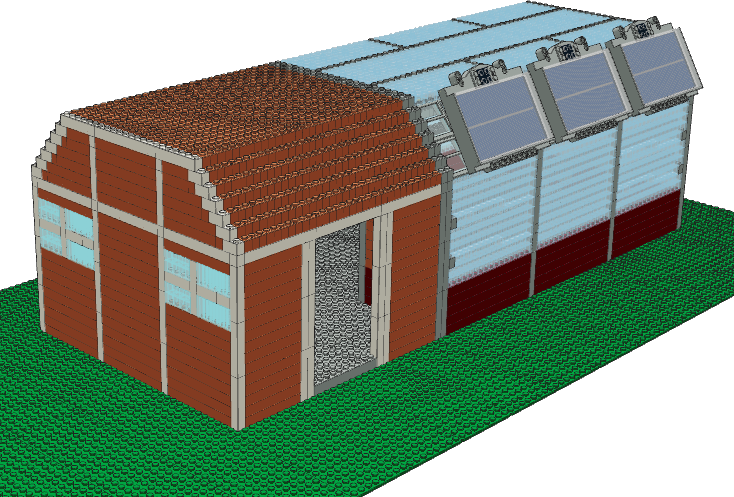
\includegraphics[width=\textwidth]{./figures/glasshouse_1.png}
        \caption{Exterior design}
        \label{fig:glasshouse_1}
    \end{subfigure}
    \hfill
    \begin{subfigure}[b]{0.3\textwidth}
        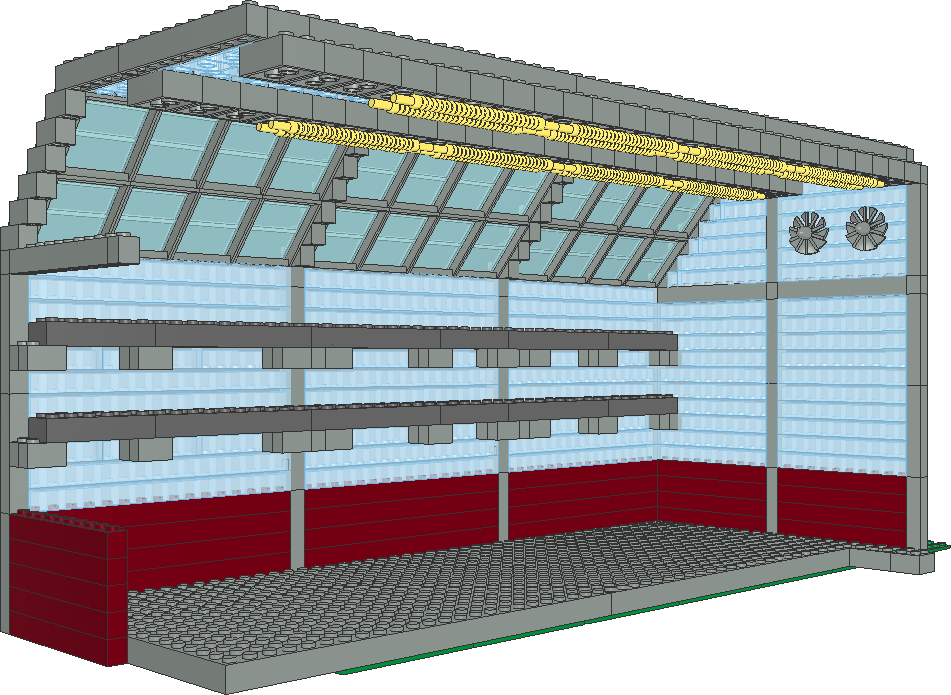
\includegraphics[width=\textwidth]{./figures/glasshouse_2.png}
        \caption{Interior design (grow area)}
        \label{fig:glasshouse_2}
    \end{subfigure}
    \hfill
    \begin{subfigure}[b]{0.3\textwidth}
        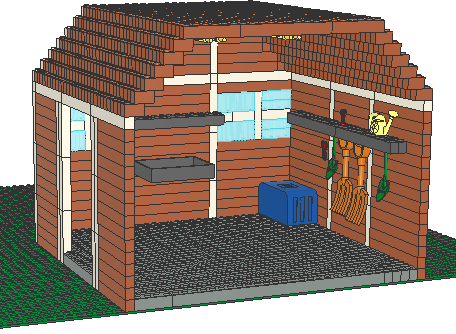
\includegraphics[width=\textwidth]{./figures/glasshouse_3.png}
        \caption{Interior design (shed area)}
        \label{fig:glasshouse_3}
    \end{subfigure}
    \caption{Mechanical design with digital LEGO bricks.}
    \label{fig:glasshouse}
\end{figure}

Besides requirements analysis and mechanical design the group was tasked with applying finite element analysis, computational fluid dynamics, and multi-physics simulation for validating selected system properties.
The group decided to apply finite element analysis for analysing the stability of the mechanical structure under snow and wind pressure, as well as computational fluid dynamics for analyzing the heat loss characteristics.
Furthermore, Figure~\ref{fig:glasshouse-sim} TODO

\begin{figure}[htbp]
    \begin{subfigure}[b]{0.56\textwidth}
        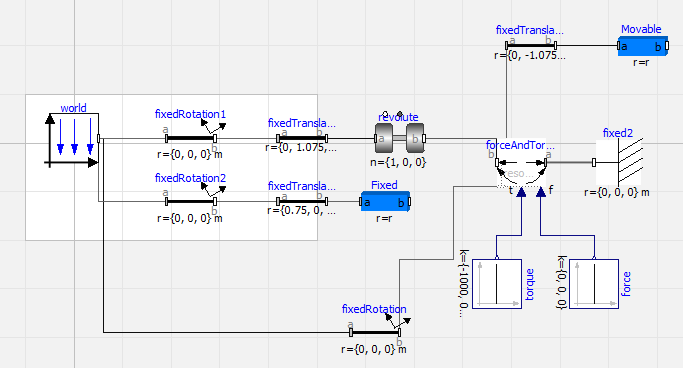
\includegraphics[width=\textwidth]{./figures/glasshouse_mechatronic_1.png}
        \caption{Component model}
        \label{fig:glasshouse-sim-1}
    \end{subfigure}
    \hfill
    \begin{subfigure}[b]{0.4\textwidth}
        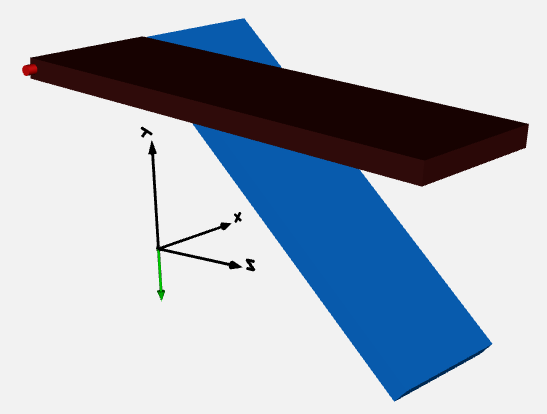
\includegraphics[width=\textwidth]{./figures/glasshouse_mechatronic_2.png}
        \caption{3D visualization}
        \label{fig:glasshouse-sim-2}
    \end{subfigure}
    \caption{Mechatronic simulation.}
    \label{fig:glasshouse-sim}
\end{figure}

TODO

\subsubsection{Paper folding machines}
\label{sec:master-system-lego}

TODO

\begin{figure}[htbp]
    \begin{subfigure}[b]{0.3\textwidth}
        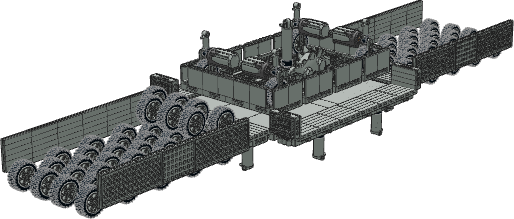
\includegraphics[width=\textwidth]{./figures/paper_1.png}
        \caption{First group}
        \label{fig:paper_1}
    \end{subfigure}
    \hfill
    \begin{subfigure}[b]{0.3\textwidth}
        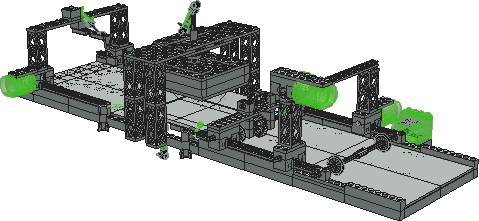
\includegraphics[width=\textwidth]{./figures/paper_2.png}
        \caption{Second group}
        \label{fig:paper_2}
    \end{subfigure}
    \hfill
    \begin{subfigure}[b]{0.3\textwidth}
        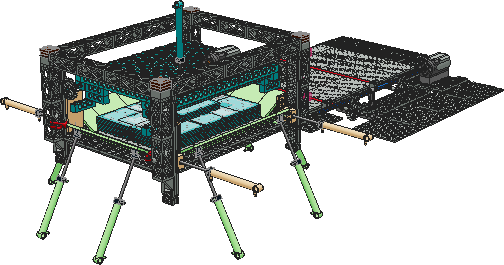
\includegraphics[width=\textwidth]{./figures/paper_3.png}
        \caption{Third group}
        \label{fig:paper_3}
    \end{subfigure}
    \caption{Mechanical designs.}
    \label{fig:paper}
\end{figure}

TODO

\begin{figure}[htbp]
    \begin{subfigure}[b]{0.45\textwidth}
        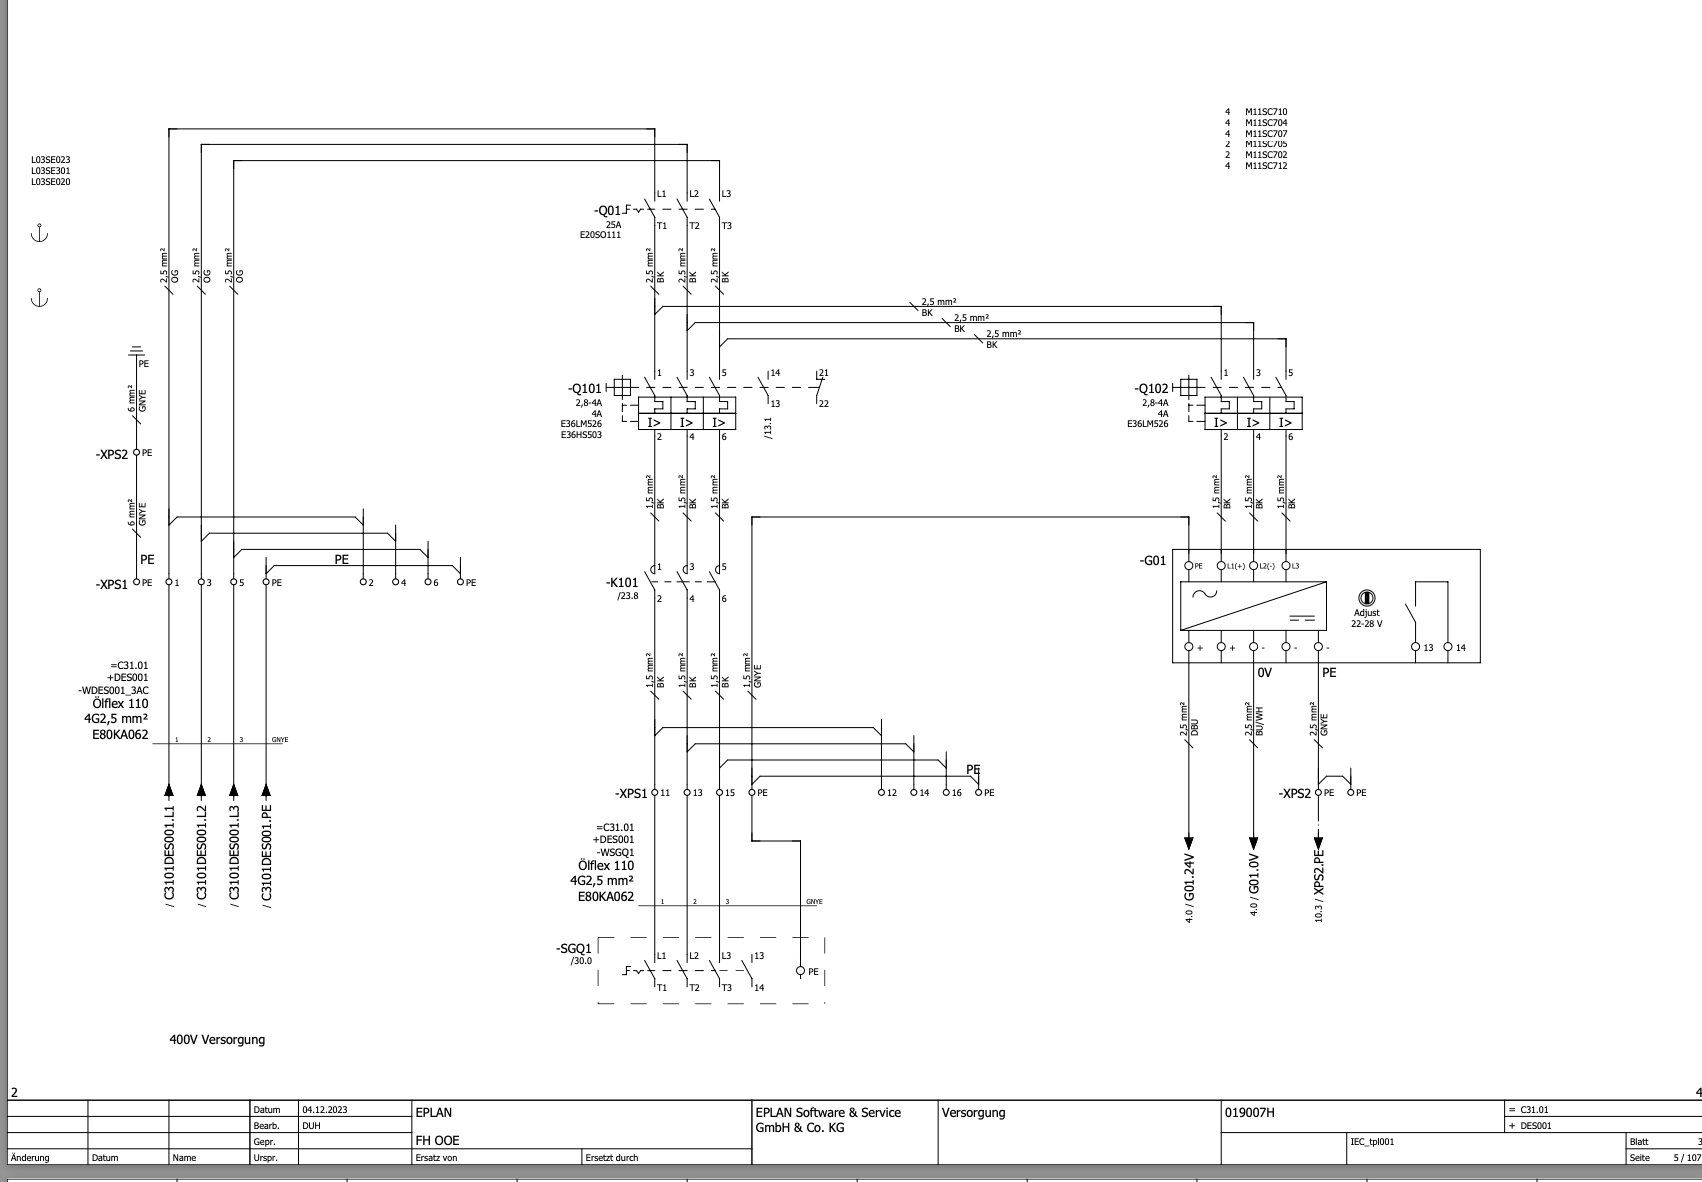
\includegraphics[width=\textwidth]{./figures/paper_electric.png}
        \caption{Electrical design}
    \end{subfigure}
    \hfill
    \begin{subfigure}[b]{0.5\textwidth}
        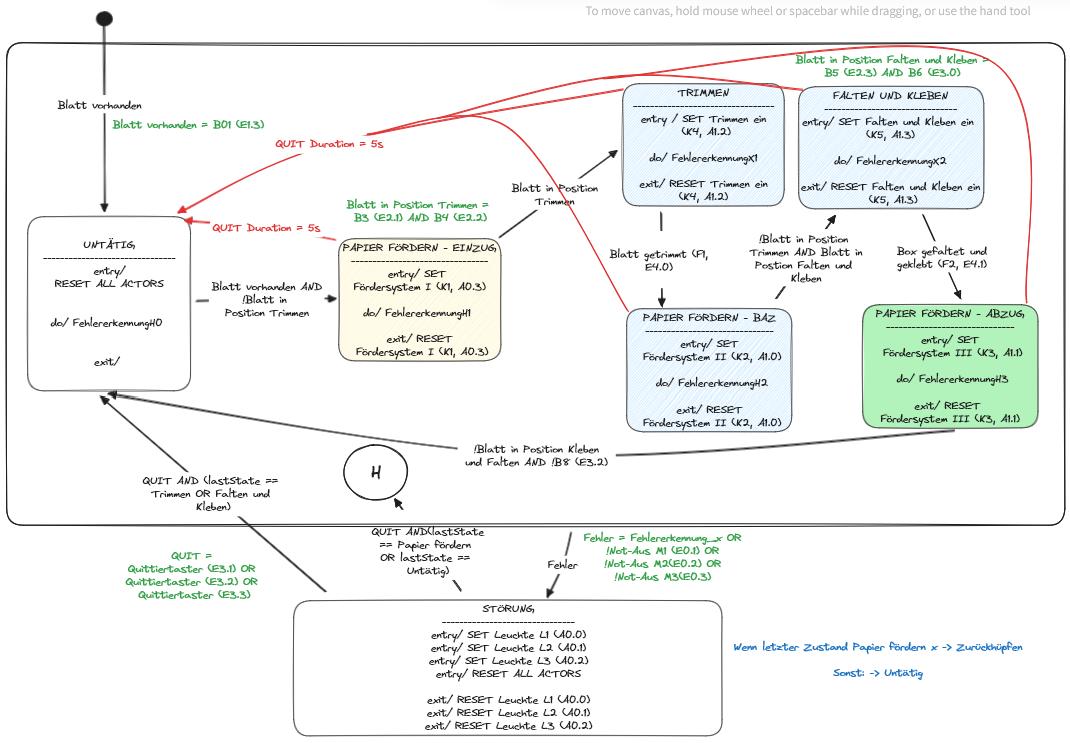
\includegraphics[width=\textwidth]{./figures/paper_control.png}
        \caption{Logical design}
    \end{subfigure}
    \caption{Electrical and logical designs.}
\end{figure}

TODO

\subsubsection{Vertical farming products}
\label{sec:master-product-classical}

TODO

\begin{figure}[htbp]
    \begin{subfigure}[b]{0.27\textwidth}
        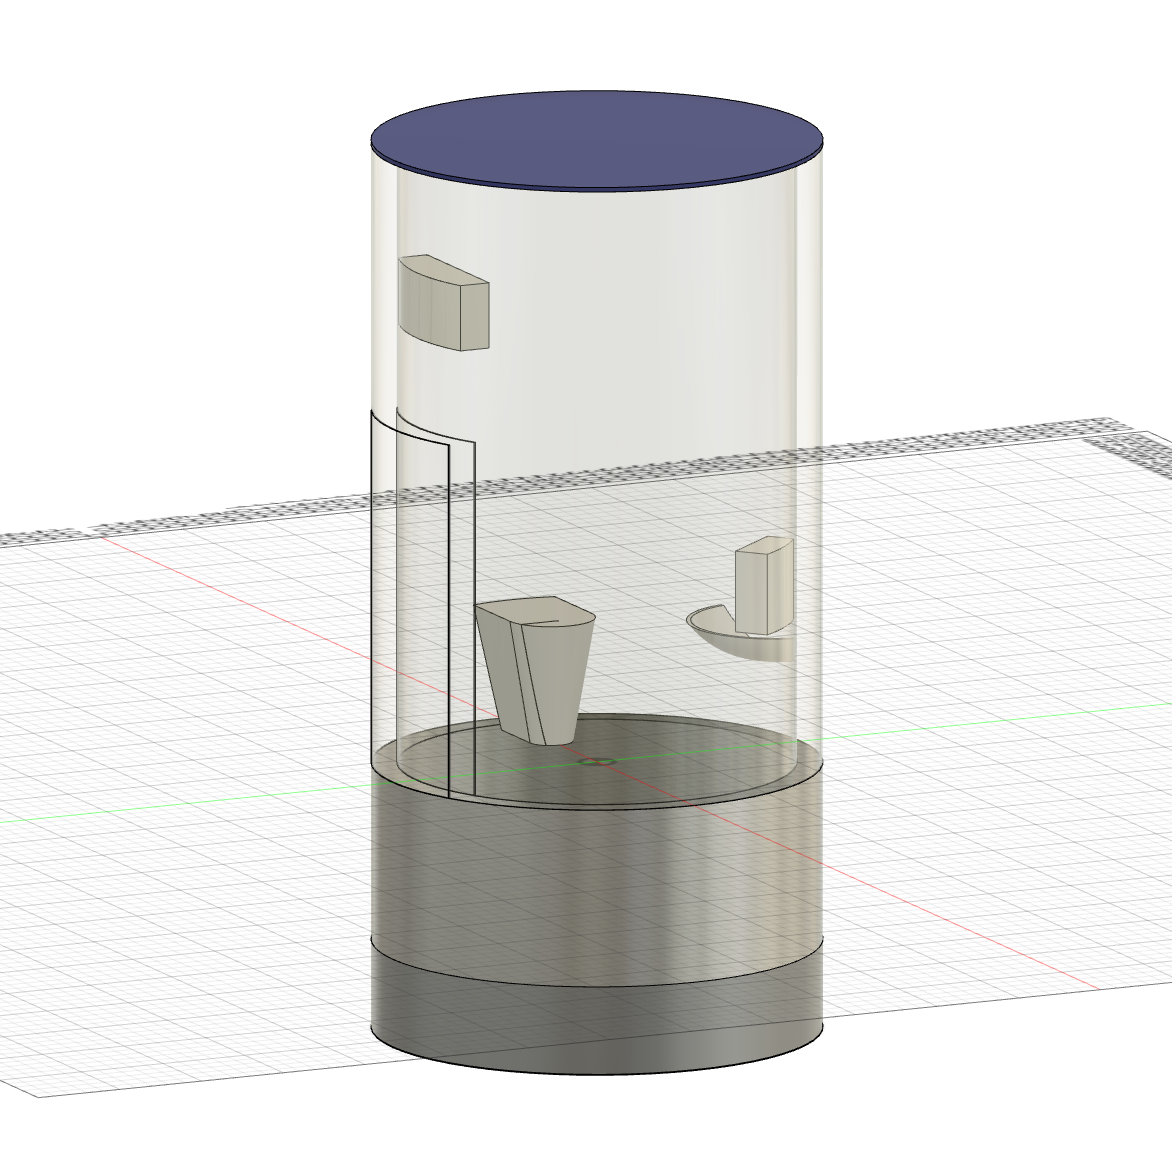
\includegraphics[width=\textwidth]{./figures/ecoflush.png}
        \caption{EcoFlush}
    \end{subfigure}
    \hfill
    \begin{subfigure}[b]{0.375\textwidth}
        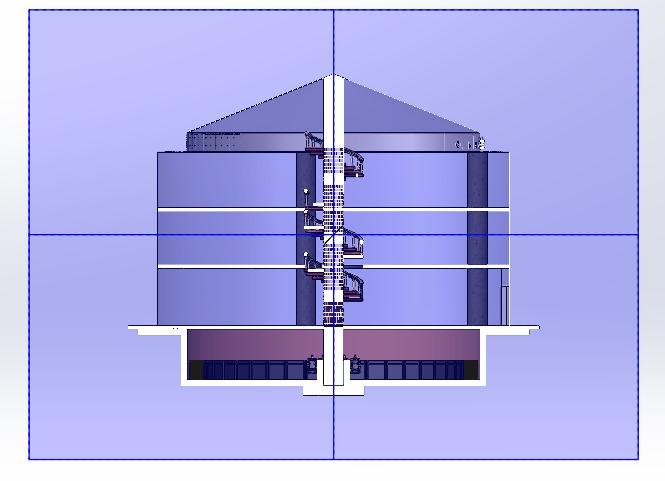
\includegraphics[width=\textwidth]{./figures/golazo-1.jpg}
        \caption{Golazo building}
    \end{subfigure}
    \hfill
    \begin{subfigure}[b]{0.27\textwidth}
        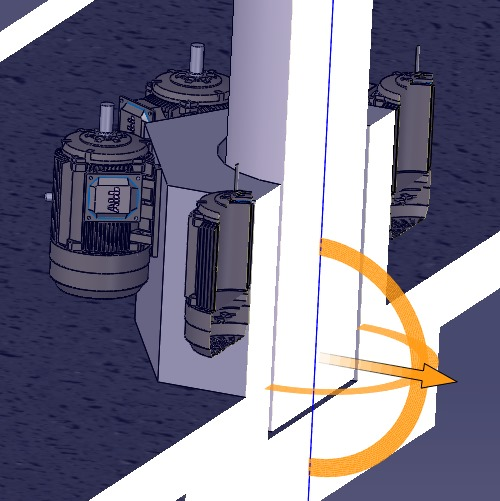
\includegraphics[width=\textwidth]{./figures/golazo-2.jpg}
        \caption{Golazo engine}
    \end{subfigure}
    \caption{Mechanical designs.}
\end{figure}

TODO

\begin{figure}
    \begin{subfigure}[b]{0.49\textwidth}
        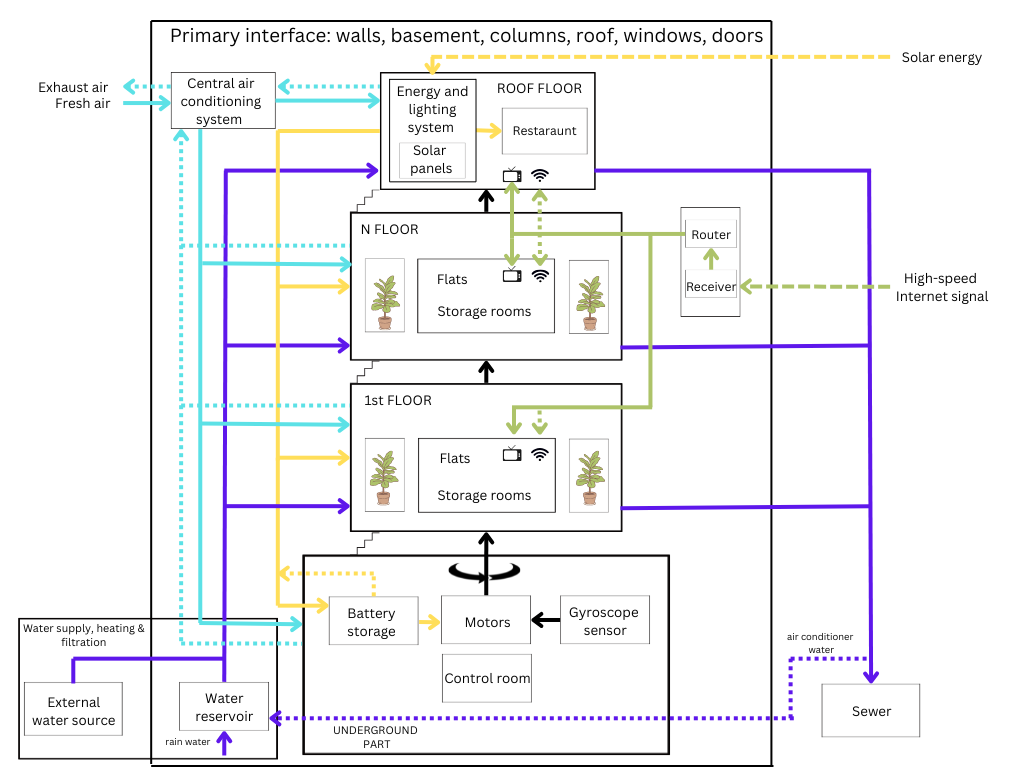
\includegraphics[width=\textwidth]{./figures/golazo-structure.png}
        \caption{Module architecture}
    \end{subfigure}
    \hfill
    \begin{subfigure}[b]{0.49\textwidth}
        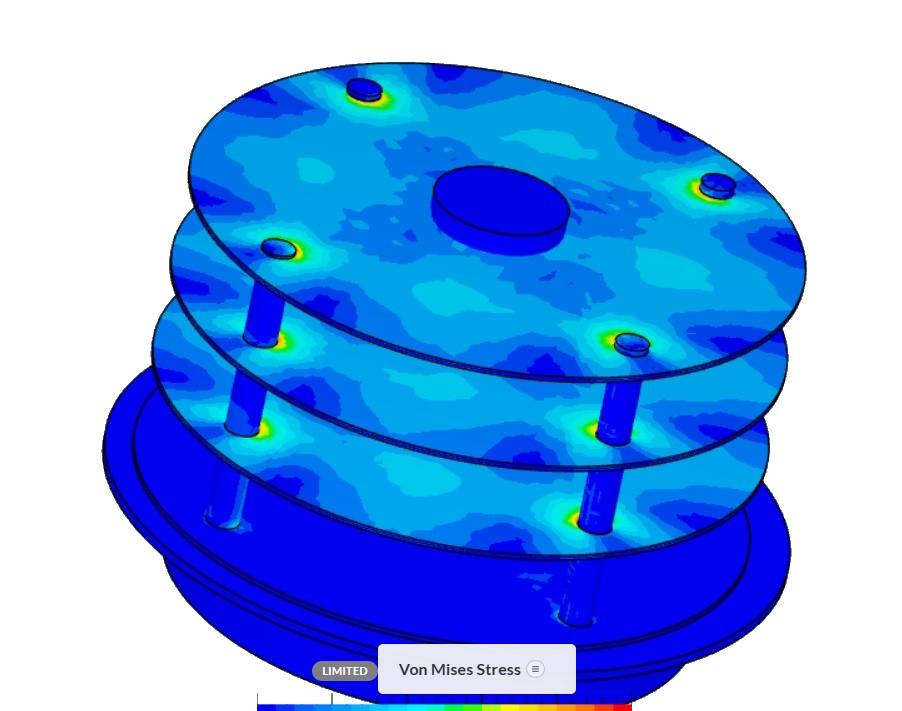
\includegraphics[width=\textwidth]{./figures/golazo-sim.jpg}
        \caption{Static simulation}
    \end{subfigure}
    \caption{Module architecture and static simulation.}
\end{figure}

TODO

\subsection{High school level}
\label{sec:school}

Section~\ref{sec:school-lego}

\subsubsection{Product design with digital LEGO}
\label{sec:school-lego}

TODO

\begin{figure}[htbp]
    \begin{subfigure}[b]{0.3\textwidth}
        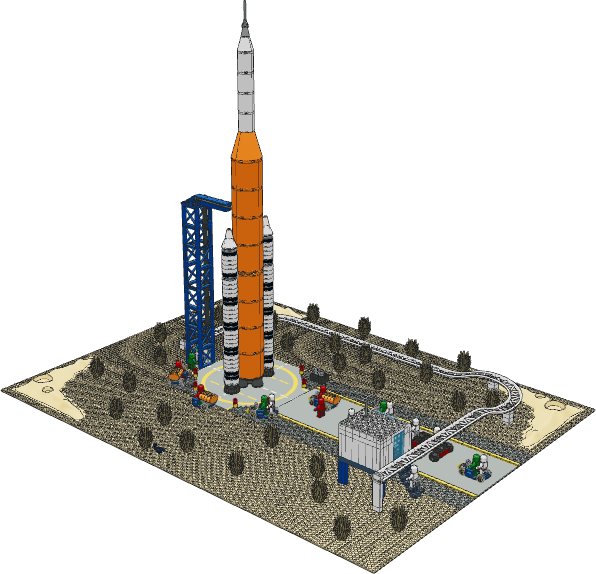
\includegraphics[width=\textwidth]{./figures/space.png}
        \caption{Space station}
        \label{fig:rocket}
    \end{subfigure}
    \hfill
    \begin{subfigure}[b]{0.3\textwidth}
        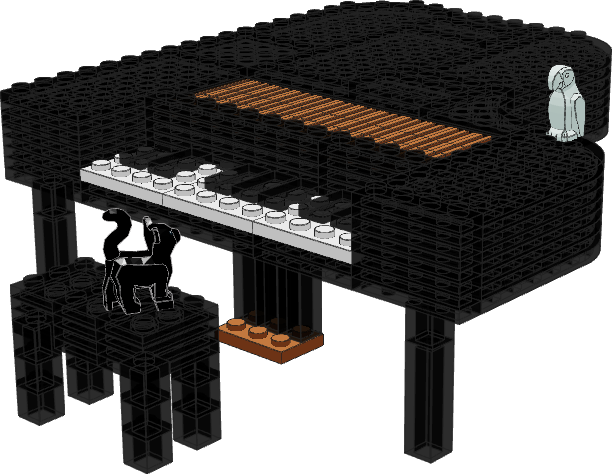
\includegraphics[width=\textwidth]{./figures/piano.png}
        \caption{Animal piano}
        \label{fig:piano}
    \end{subfigure}
    \hfill
    \begin{subfigure}[b]{0.3\textwidth}
        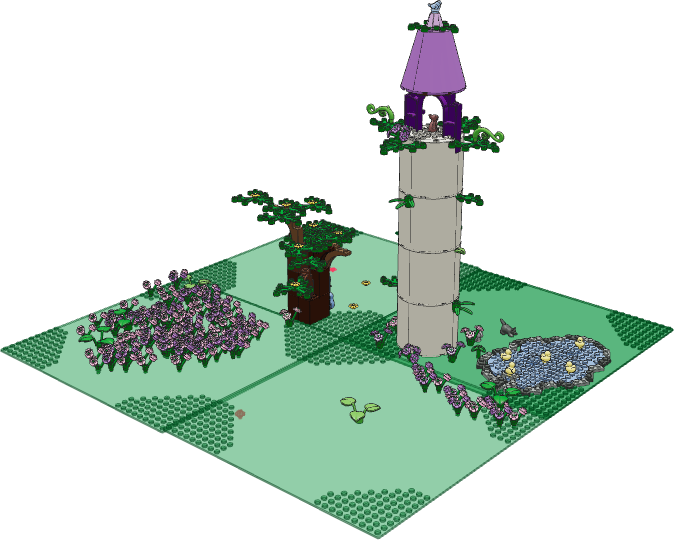
\includegraphics[width=\textwidth]{./figures/rapunzel.png}
        \caption{Rapunzel tower}
        \label{fig:rapunzel}
    \end{subfigure}
    \caption{Product designs.}
    \label{fig:kinderuni}
\end{figure}

TODO

\begin{figure}[htbp]
    \begin{subfigure}[b]{0.3\textwidth}
        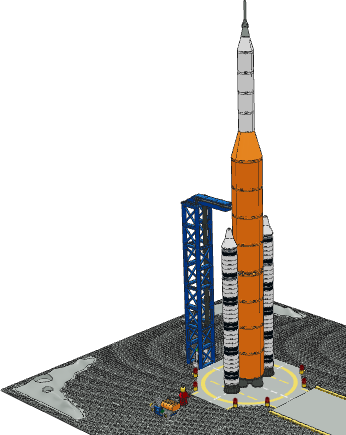
\includegraphics[width=\textwidth]{./figures/space_rocket.png}
        \caption{Rocket}
    \end{subfigure}
    \hfill
    \begin{subfigure}[b]{0.65\textwidth}
        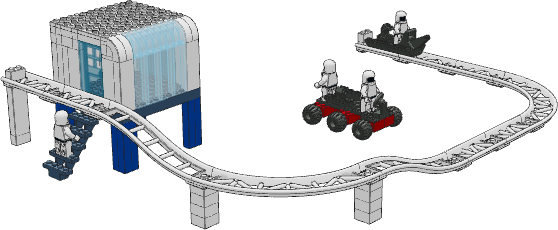
\includegraphics[width=\textwidth]{./figures/space_station.png}
        \caption{Station}
    \end{subfigure}
    \caption{Product components.}
\end{figure}

TODO

\section{Evaluation results}
\label{sec:discussion}

TODO

\section{Conclusions}
\label{sec:conclusion}

TODO

\paragraph{Summary}

TODO

\paragraph{Outlook}

TODO

\begin{Backmatter}

\bibliography{main}
\bibliographystyle{plainnat}

\end{Backmatter}

\end{document}